\documentclass[11pt,a4paper]{article}
\usepackage[utf8]{inputenc}
\usepackage[T1]{fontenc}
\usepackage{amsmath,amssymb}
\usepackage{geometry,enumitem,booktabs,xcolor}
\usepackage{tcolorbox}
\usepackage{tikz}
\usetikzlibrary{arrows.meta,positioning,calc,decorations.pathreplacing}
\usepackage{hyperref}

\geometry{margin=2cm}
\hypersetup{colorlinks=true,linkcolor=blue!60!black,urlcolor=blue!70!black}
\tcbuselibrary{skins}
\newcommand{\PsiNN}{$\Psi$-NN}
\newcommand{\R}{\mathbf{R}}
\newcommand{\W}{\mathbf{W}}

\title{\textbf{Schematic Explanation}\\[3pt]
\large\PsiNN{}: Automatic Network Structure Discovery of PINNs\\
via Knowledge Distillation\\[2pt]
\normalsize Liu et al.\ -- \textit{Nature Communications} (2025) 16:9558}
\author{Meeting 3 -- PFE}
\date{\today}

\begin{document}
\maketitle
\tableofcontents
\newpage

%=================================================================
\section{The Problem in One Diagram}
%=================================================================

\begin{center}
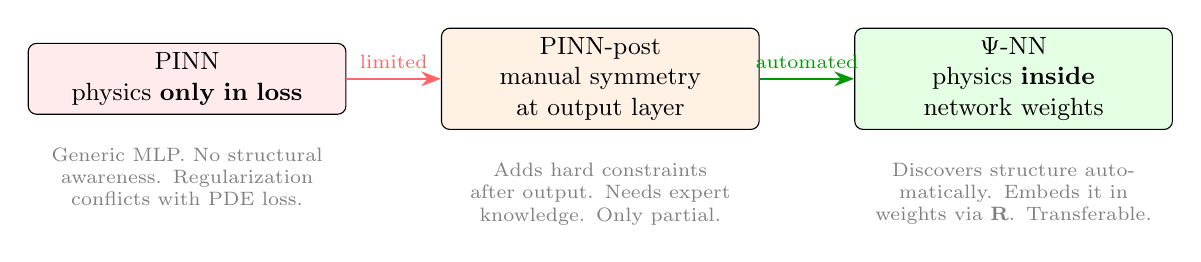
\begin{tikzpicture}[
    every node/.style={font=\small},
    mbox/.style={draw,rounded corners=3pt,minimum height=0.9cm,align=center,text width=3.8cm},
    arr/.style={-{Stealth[length=2.5mm]},thick},
    lbl/.style={font=\scriptsize,midway,above}
]
% Row 1: the problem
\node[mbox,fill=red!8] (pinn)  {PINN\\physics \textbf{only in loss}};
\node[mbox,fill=orange!10,right=1.2cm of pinn] (post) {PINN-post\\manual symmetry\\at output layer};
\node[mbox,fill=green!10,right=1.2cm of post] (psi)  {\PsiNN{}\\physics \textbf{inside}\\network weights};

\draw[arr,red!60]   (pinn) -- node[lbl]{\color{red!60}limited} (post);
\draw[arr,green!60!black] (post) -- node[lbl]{\color{green!60!black}automated} (psi);

% Annotations below
\node[below=0.3cm of pinn,font=\scriptsize,text width=3.8cm,align=center,gray] {Generic MLP. No structural awareness. Regularization conflicts with PDE loss.};
\node[below=0.3cm of post,font=\scriptsize,text width=3.8cm,align=center,gray] {Adds hard constraints after output. Needs expert knowledge. Only partial.};
\node[below=0.3cm of psi,font=\scriptsize,text width=3.8cm,align=center,gray]  {Discovers structure automatically. Embeds it in weights via $\R$. Transferable.};
\end{tikzpicture}
\end{center}

%=================================================================
\section{The \PsiNN{} Pipeline (3 Stages)}
%=================================================================

\begin{figure}[h!]
\centering
\begin{tikzpicture}[
    stage/.style={draw,rounded corners=5pt,minimum width=11.5cm,minimum height=2.4cm,align=left,inner sep=8pt},
    stitle/.style={font=\bfseries\small,anchor=north west},
    arr/.style={-{Stealth[length=3mm]},very thick,blue!50!black},
    every node/.style={font=\small}
]

% Stage 1
\node[stage,fill=red!5] (s1) at (0,0) {};
\node[stitle] at (s1.north west) {Stage 1: Distillation};
\node[anchor=north west,text width=10.5cm] at ($(s1.north west)+(0.1,-0.55)$) {%
\begin{tikzpicture}[
    bx/.style={draw,rounded corners=2pt,minimum height=0.7cm,align=center,font=\footnotesize},
    ar/.style={-{Stealth[length=2mm]},thick}
]
\node[bx,fill=red!15,text width=2.5cm] (teacher) {Teacher (PINN)\\$\mathcal{L}= \text{MSE}_{\text{PDE}}+\text{MSE}_{\text{BC}}$};
\node[bx,fill=orange!12,text width=2.5cm,right=1.5cm of teacher] (student) {Student (MLP)\\$\mathcal{L}= \text{MSE}_T + \lambda\|\theta\|_2^2$};
\node[right=0.6cm of student,font=\footnotesize,text width=3.5cm] (note) {No PDE loss on student $\Rightarrow$ L2 reg.\ does \textbf{not} conflict with physics.};
\draw[ar] (teacher) -- node[above,font=\scriptsize]{output $\tilde{u}_T$} (student);
\end{tikzpicture}};

% Stage 2
\node[stage,fill=yellow!5,below=0.5cm of s1] (s2) {};
\node[stitle] at (s2.north west) {Stage 2: Structure Extraction};
\node[anchor=north west,text width=10.5cm] at ($(s2.north west)+(0.1,-0.55)$) {%
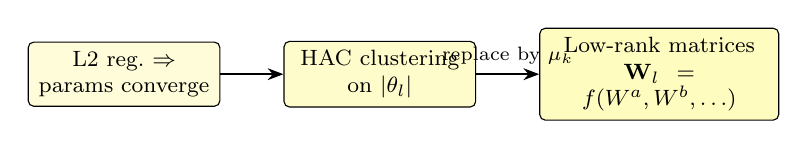
\begin{tikzpicture}[
    bx/.style={draw,rounded corners=2pt,minimum height=0.7cm,align=center,font=\footnotesize},
    ar/.style={-{Stealth[length=2mm]},thick}
]
\node[bx,fill=yellow!15,text width=2.2cm] (reg) {L2 reg.\ $\Rightarrow$\\params converge};
\node[bx,fill=yellow!20,text width=2.2cm,right=0.8cm of reg] (hac) {HAC clustering\\on $|\theta_l|$};
\node[bx,fill=yellow!25,text width=2.8cm,right=0.8cm of hac] (lr) {Low-rank matrices\\$\W_l = f(W^a, W^b,\ldots)$};
\draw[ar] (reg) -- (hac);
\draw[ar] (hac) -- node[above,font=\scriptsize]{replace by $\mu_k$} (lr);
\end{tikzpicture}};

% Stage 3
\node[stage,fill=green!5,below=0.5cm of s2] (s3) {};
\node[stitle] at (s3.north west) {Stage 3: Reconstruction};
\node[anchor=north west,text width=10.5cm] at ($(s3.north west)+(0.1,-0.55)$) {%
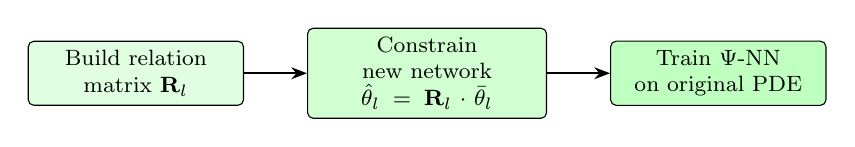
\begin{tikzpicture}[
    bx/.style={draw,rounded corners=2pt,minimum height=0.7cm,align=center,font=\footnotesize},
    ar/.style={-{Stealth[length=2mm]},thick}
]
\node[bx,fill=green!12,text width=2.5cm] (rel) {Build relation\\matrix $\R_l$};
\node[bx,fill=green!18,text width=2.8cm,right=0.8cm of rel] (embed) {Constrain new network\\$\hat{\theta}_l = \R_l \cdot \bar{\theta}_l$};
\node[bx,fill=green!25,text width=2.5cm,right=0.8cm of embed] (train) {Train \PsiNN{}\\on original PDE};
\draw[ar] (rel) -- (embed);
\draw[ar] (embed) -- (train);
\end{tikzpicture}};

% Arrows between stages
\draw[arr] (s1.south) -- (s2.north);
\draw[arr] (s2.south) -- (s3.north);

\end{tikzpicture}
\caption{Complete \PsiNN{} pipeline.}
\end{figure}

%=================================================================
\section{Stage 1 -- Distillation: How and Why}
%=================================================================

\textbf{Core problem:} Adding regularization (L1, L2, GrOWL) to a PINN \emph{increases} the loss because the regularization gradient opposes the PDE gradient.

\textbf{Solution:} Separate the two tasks into two networks:

\begin{center}
\renewcommand{\arraystretch}{1.3}
\begin{tabular}{@{}l l l@{}}
\toprule
& \textbf{Teacher} & \textbf{Student} \\
\midrule
Architecture & MLP & MLP (same size) \\
Loss & $\text{MSE}_{\text{PDE}} + \text{MSE}_{\text{BC}} + \text{MSE}_{\text{data}}$ & $\text{MSE}_T + \displaystyle\sum_l \omega_l\|\theta_l\|_2^2$ \\
PDE derivatives & Yes (high-order) & \textbf{None} \\
Regularization & None & L2 (drives convergence) \\
Role & Learn the physics & Learn the output + reveal structure \\
\bottomrule
\end{tabular}
\end{center}

\textbf{Student loss:}
\begin{equation}
\mathcal{L}_{\text{student}} = \frac{1}{M_T}\sum_{i=1}^{M_T} \big|\tilde{u}_T^{(i)} - \tilde{u}_S^{(i)}\big|^2 + \sum_{l=1}^{L} \omega_l \|\theta_l\|_2^2
\end{equation}

%=================================================================
\section{Stage 2 -- Structure Extraction: How and Why}
%=================================================================

\subsection{Theoretical foundation}

\begin{tcolorbox}[colback=yellow!6,colframe=orange!60!black,title={\small Theorem 1: Equivalent parameters converge}]
\small Parameters $\theta_1,\dots,\theta_n$ in the same layer that play \textbf{equivalent roles} $\xrightarrow{\text{L2 reg.}}$ converge to the \textbf{same value}.
\end{tcolorbox}

\begin{tcolorbox}[colback=yellow!6,colframe=orange!60!black,title={\small Theorem 2: Symmetric parameters converge in absolute value}]
\small If $|\theta_i|=|\theta_j|$ (possibly with different signs) $\xrightarrow{\text{L2 reg.}}$ their absolute values converge.
\end{tcolorbox}

\subsection{Extraction steps}

\begin{enumerate}[leftmargin=1.8em,itemsep=2pt]
\item For each layer $l$, compute $|\theta_l|$.
\item Run HAC (Hierarchical Agglomerative Clustering) $\longrightarrow$ $K$ clusters $\{C_1,\dots,C_K\}$.
\item Replace each weight by its cluster center, keeping sign:
\begin{equation}
    \theta_{l,i}^{\text{new}} = \operatorname{sgn}(\theta_{l,i})\cdot\mu_k, \quad \theta_{l,i}\in C_k
\end{equation}
\item The weight matrices now show a \textbf{low-rank pattern}: each full matrix is assembled from a few independent sub-matrices via sharing, sign flips, and permutations.
\end{enumerate}

\subsection{Laplace example -- extracted matrices}

\begin{equation}
\W_1\!=\!\begin{bmatrix} W_1^a & W_1^b \\ -W_1^a & -W_1^b \end{bmatrix}\!,\;
\W_2\!=\!\begin{bmatrix} -W_2^a & -W_2^b \\ W_2^b & W_2^a \end{bmatrix}\!,\;
\W_3\!=\!\begin{bmatrix} W_3^a & W_3^a \end{bmatrix}
\end{equation}

\begin{center}
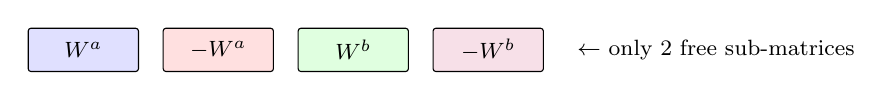
\begin{tikzpicture}[
    every node/.style={font=\footnotesize},
    mat/.style={draw,minimum width=1.4cm,minimum height=0.55cm,align=center,rounded corners=1pt}
]
\node[mat,fill=blue!12] (wa) {$W^a$};
\node[mat,fill=red!12,right=0.3cm of wa] (mwa) {$-W^a$};
\node[mat,fill=green!12,right=0.3cm of mwa] (wb) {$W^b$};
\node[mat,fill=purple!12,right=0.3cm of wb] (mwb) {$-W^b$};
\node[right=0.3cm of mwb] {$\leftarrow$ only 2 free sub-matrices};
\end{tikzpicture}
\end{center}

%=================================================================
\section{Stage 3 -- Final Model Build: How and Why}
%=================================================================

\subsection{The Relation Matrix $\mathbf{R}$}
The core innovation of \PsiNN{} is the mathematical formalization of the discovered structure using a \textbf{Relation Matrix} $\mathbf{R}$.

In a standard neural network, a weight matrix $\mathbf{W} \in \mathbb{R}^{m \times n}$ has $m \times n$ independent parameters. In \PsiNN{}, we decompose this matrix:
\begin{equation}
    \text{vec}(\mathbf{W}_l) = \mathbf{R}_l \cdot \bar{\mathbf{\theta}}_l
\end{equation}
Where:
\begin{itemize}
    \item $\bar{\mathbf{\theta}}_l \in \mathbb{R}^{K}$ is a vector containing only the $K$ unique cluster centers (the independent parameters).
    \item $\mathbf{R}_l$ is a constant, sparse matrix that maps each unique parameter to its corresponding positions in the full weight matrix, including sign flips ($+1, -1, 0$).
\end{itemize}

\subsection{Physics-Embedded Architecture}
By training the final model via $\bar{\mathbf{\theta}}_l$, the network is structurally incapable of violating the discovered symmetries.
\begin{enumerate}
    \item \textbf{Reduced Parameter Space:} Since $K \ll m \times n$, the training is faster and less prone to local minima.
    \item \textbf{Internalized Physics:} Unlike standard PINNs where physics is a "soft" penalty in the loss function ($\mathcal{L}_{PDE}$), \PsiNN{} treats physics as a "hard" constraint in the weights.
    \item \textbf{Convergence Stability:} This architecture prevents the "Gradient Conflict" frequently observed when the PDE loss and data loss compete for the same weights.
\end{enumerate}

\section{Application: Offshore Wind Piles}
Integrating \PsiNN{} into the soil-structure interaction model allows for:
\begin{itemize}
    \item \textbf{Automated Domain Coupling:} The relation matrix $\mathbf{R}$ can identify shared behavioral patterns between different "slots" (e.g., Soil and Structural).
    \item \textbf{Superior Generalization:} Because the architecture is physically informed, it performs better on unseen storm scenarios where standard MLPs might produce non-physical oscillations.
\end{itemize}
\end{document}


$\R$ encodes three types of parameter relationships:

\begin{center}
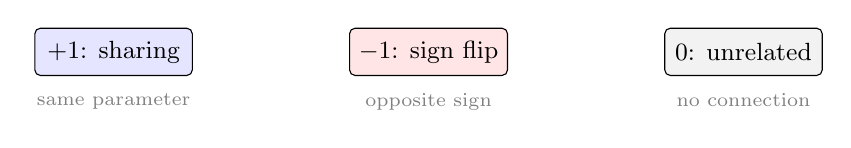
\begin{tikzpicture}[
    every node/.style={font=\small},
    box/.style={draw,rounded corners=2pt,minimum height=0.6cm,minimum width=2cm,align=center}
]
\node[box,fill=blue!10]   (s) at (0,0) {$+1$: sharing};
\node[box,fill=red!10]    (r) at (4,0) {$-1$: sign flip};
\node[box,fill=gray!10]   (u) at (8,0) {$0$: unrelated};
\node[below=0.1cm of s,font=\scriptsize,gray] {same parameter};
\node[below=0.1cm of r,font=\scriptsize,gray] {opposite sign};
\node[below=0.1cm of u,font=\scriptsize,gray] {no connection};
\end{tikzpicture}
\end{center}

Row permutations in $\R$ encode \textbf{swapping} relationships.

\subsection{Laplace example -- 2nd hidden layer}

\begin{equation}
\underbrace{\R_2 = \begin{bmatrix} -1 & 0 \\ 0 & -1 \\ 0 & 1 \\ 1 & 0 \end{bmatrix}}_{\text{encodes structure}}
\;\times\;
\underbrace{\begin{bmatrix} \hat{\theta}_2^a & 0 \\ 0 & \hat{\theta}_2^b \end{bmatrix}}_{\text{free params (only 2)}}
\;=\;
\underbrace{\begin{bmatrix} -\hat{\theta}_2^a & 0 \\ 0 & -\hat{\theta}_2^b \\ 0 & \hat{\theta}_2^b \\ \hat{\theta}_2^a & 0 \end{bmatrix}}_{\text{full constrained matrix}}
\end{equation}

\subsection{Reconstruction procedure}

\begin{center}
\begin{tikzpicture}[
    step/.style={draw,rounded corners=3pt,fill=green!8,minimum height=0.7cm,text width=3.2cm,align=center,font=\footnotesize},
    arr/.style={-{Stealth[length=2mm]},thick}
]
\node[step] (a) at (0,0) {Sparsify\\(zero out noise)};
\node[step,right=0.5cm of a] (b) {Reinitialize\\salient params};
\node[step,right=0.5cm of b] (c) {Apply $\R$\\(constrain weights)};
\node[step,right=0.5cm of c] (d) {Train \PsiNN{}\\on original PDE};
\draw[arr](a)--(b); \draw[arr](b)--(c); \draw[arr](c)--(d);
\end{tikzpicture}
\end{center}

%=================================================================
\section{Why It Works: Symmetry Proof (Laplace)}
%=================================================================

With the extracted structure, the two outputs of the last hidden layer are:
\begin{align}
u^a(x_1,x_2) &= \tanh\!\big(W_2^a\,\sigma_+ + W_2^b\,(\sigma_- + b_2^a)\big) \\
u^b(x_1,x_2) &= \tanh\!\big(W_2^b\,\sigma_+ + W_2^a\,(\sigma_- + b_2^a)\big)
\end{align}
where $\sigma_\pm = \tanh(W_1^a x_1 \pm W_1^b x_2 + b_1^a)$.

Replacing $x_2\to -x_2$ swaps $\sigma_+\leftrightarrow\sigma_-$, hence:
\begin{equation}
\boxed{u^a(x_1,x_2) = u^b(x_1,-x_2)}
\end{equation}

Final output:
\begin{equation}
u(x_1,x_2) = W_3^a\big(u^a(x_1,x_2)+u^a(x_1,-x_2)\big) \;\Longrightarrow\; u(x_1,x_2)=u(x_1,-x_2)
\end{equation}

The network \textbf{inherently satisfies} the Laplace symmetry -- no post-processing needed.

%=================================================================
\section{Numerical Results}
%=================================================================

\subsection{Four benchmark cases}

\begin{center}
\renewcommand{\arraystretch}{1.25}
\begin{tabular}{@{}l l l l@{}}
\toprule
\textbf{Case} & \textbf{PDE} & \textbf{Symmetry found} & \textbf{Special feature} \\
\midrule
Laplace    & $\nabla^2 u=0$ & $u(x_1,x_2)=u(x_1,-x_2)$ & Full extraction walkthrough \\
Burgers    & $u_t+uu_x+\lambda_1 u_{xx}=0$ & Antisymmetric & Inverse problem; transfers across $\nu$ \\
Poisson    & $\nabla^2 u=f$ (4 frequencies) & $\mathbb{Z}_2\!\times\!\mathbb{Z}_2$ equivariance & Low-freq $\to$ high-freq transfer \\
Cylinder   & Navier--Stokes & Opposite symmetries on $u,v,p$ & Multi-output; reuses prior structures \\
\bottomrule
\end{tabular}
\end{center}

\subsection{$L_2$ error comparison}

\begin{center}
\renewcommand{\arraystretch}{1.2}
\begin{tabular}{@{}l c c c@{}}
\toprule
\textbf{Problem} & \textbf{PINN} & \textbf{PINN-post} & \textbf{\PsiNN{}} \\
\midrule
Laplace ($\times10^{-4}$)  & 11.59 & 4.017 & \textbf{0.742} \\
Burgers ($\times10^{-2}$)  & 14.47 & 3.014 & \textbf{1.287} \\
Poisson ($\times10^{-2}$)  & 2.633 & 2.563 & \textbf{2.464} \\
Flow $p$ ($\times10^{-4}$) & 14.89 & 11.78 & \textbf{7.838} \\
Flow $u$ ($\times10^{-4}$) & 1.981 & 1.904 & \textbf{1.854} \\
Flow $v$ ($\times10^{-5}$) & 1.984 & 1.896 & \textbf{1.765} \\
\bottomrule
\end{tabular}
\end{center}

\PsiNN{} achieves the \textbf{lowest error in every case}.

\subsection{Burgers inverse problem -- parameter estimation}

\begin{center}
\renewcommand{\arraystretch}{1.2}
\begin{tabular}{@{}l c c c c@{}}
\toprule
& \textbf{Truth} & \textbf{PINN} & \textbf{PINN-post} & \textbf{\PsiNN{}} \\
\midrule
$\nu_1\!\cdot\!\pi$ ($\times10^{-2}$) & 1 & 2.820 & 1.898 & \textbf{1.465} \\
$\nu_2\!\cdot\!\pi$ ($\times10^{-2}$) & 4 & 6.625 & 4.960 & \textbf{4.084} \\
$\nu_3\!\cdot\!\pi$ ($\times10^{-2}$) & 8 & 9.705 & 0.885 & \textbf{6.673} \\
\bottomrule
\end{tabular}
\end{center}

Same \PsiNN{} structure used for all three $\nu$ values -- no retraining needed.

%=================================================================
\section{Advantages vs.\ Limitations}
%=================================================================

\begin{center}
\renewcommand{\arraystretch}{1.3}
\begin{tabular}{@{}p{6.5cm} p{6.5cm}@{}}
\toprule
\textbf{Advantages} & \textbf{Limitations} \\
\midrule
Automatic discovery (no expert priors) & Requires at least partially known PDEs \\
Physics \textit{inside} weights $\Rightarrow$ strict satisfaction & Currently validated on 3-layer MLP + $\tanh$ only \\
Interpretable (low-rank matrices $\leftrightarrow$ symmetries) & Limited to sign \& permutation symmetries \\
Fewer free parameters $\Rightarrow$ faster training & Extension to Transformers is future work \\
Transferable across parameters \& problems & Complex symmetries (rotation, Noether) not yet handled \\
\bottomrule
\end{tabular}
\end{center}

%=================================================================
\section{Key Equations -- Quick Reference}
%=================================================================

\begin{tcolorbox}[colback=blue!3,colframe=blue!40!black]
\renewcommand{\arraystretch}{1.8}
\begin{tabular}{@{}l l@{}}
\textbf{Distillation loss} & $\displaystyle\text{MSE}_T = \frac{1}{M_T}\sum_{i=1}^{M_T}|\tilde{u}_T^{(i)}-\tilde{u}_S^{(i)}|^2$ \\
\textbf{L2 regularization} & $\displaystyle\Omega(\theta_S) = \sum_{l=1}^{L}\omega_l\|\theta_l\|_2^2$ \\
\textbf{Clustering replacement} & $\theta_{l,i}^{\text{new}} = \operatorname{sgn}(\theta_{l,i})\cdot\mu_k \;\;(\theta_{l,i}\in C_k)$ \\
\textbf{Reconstruction} & $\hat{\theta}_l = \R_l\cdot\bar{\theta}_l \;\;$ where $\R_l\in\{-1,0,+1\}^{n\times K}$ \\
\end{tabular}
\end{tcolorbox}

\end{document}
